\begin{theorem}
\label{3-thm:value_iteration_quasipoly}
There exists a value iteration algorithm for solving parity games in time 
\[
O\left(nm \log(n) \log(d) \cdot  \binom{\lceil \log(n) \rceil + d/2 - 1}{\lceil \log(n) \rceil} \right),
\]
which is quasipolynomial in general and polynomial if $d = O(\log(n))$.
The space complexity of the algorithm is $O(m + n \log(d))$.
\end{theorem}

We rely on the high-level presentation of value iteration algorithms given in \cref{1-sec:value_iteration}.
Let $\game = (\arena,\Parity[\col])$ a parity game with $n$ vertices and priorities in $[1,d]$,
and without loss of generality $d$ is even.

The first step is to define a notion of value function $\val^\game : V \to Y$ with $(Y,\le)$ a lattice satisfying the characterisation principle:
for all vertices $v$ we have that Eve wins from $v$ if and only if $\val^\game(v) \neq \bot$, where $\bot$ is the least element in $Y$.
The goal of the algorithm is to compute $\val^\game$, from which we then easily obtain the winning region thanks to the characterisation principle.

To set the machinery of value iteration algorithms in motion we can either construct $\val^\game$ as the unique fixed point of a contracting operator using Banach's fixed point theorem or the greatest fixed point of a monotonic operator using Kleene's fixed point theorem.

Let us here follow the second approach. 
We let $F_V$ be the lattice of functions $V \to Y$ equipped with the componentwise order induced by $Y$.
We are looking for a monotonic function $\delta : Y \times [1,d] \to Y$ inducing the operator $\Op : F_V \to F_V$ defined by:
\[
\Op(\mu)(v) = 
\begin{cases}
\max \set{\delta( \mu(v'), \col(v)) : (v,v') \in E} & \text{ if } v \in \VE, \\
\min \set{\delta( \mu(v'), \col(v)) : (v,v') \in E} & \text{ if } v \in \VA,
\end{cases}
\]
such that $\val^\game$ is the greatest fixed point of $\Op$.
The algorithm would then simply use \cref{1-thm:kleene} to compute $\val^\game$ by iterating the operator $\Op$.

Let us look at this question using the notion of progress measures, which are post-fixed points of $\Op$,
meaning $\mu$ such that $\mu \le \Op(\mu)$. 
Since the greatest fixed point of $\Op$ is also its greatest post-fixed point, an equivalent formulation of the characterisation principle above reads: for all vertices $v$ we have that Eve wins from $v$ if and only if there exists a progress measure $\mu$ such that $\mu(v) \neq \bot$.

To summarise this discussion, we are looking for a lattice $(Y,\le)$ and a monotonic function $\delta : Y \times [1,d] \to Y$ 
such that for all parity games $\Game$ with $n$ vertices and priorities in $[1,d]$, 
for all vertices $v$ we have that Eve wins from $v$ if and only if there exists a progress measure $\mu$ such that $\mu(v) \neq \bot$.
Our next step is to show how the notion of universal trees provides a class of solutions to this problem.
%\footnote{One can even show that any solution is equivalent to a universal tree, but we will not prove it in this chapter.}

\subsubsection*{Universal trees}
The trees we consider have three properties: 
they are rooted, every leaf has the same depth, and the children of a node are totally ordered.
Formally, a tree of height $0$ is a leaf,
and a tree $t$ of height $h + 1$ is an ordered list $[t_1,\dots,t_k]$ of subtrees each of height $h$.

We consider two parameters for trees: the height, and the size which is defined to be the number of branches (equivalently, the number of leaves).
All trees we consider have height $h = d/2$.

\begin{figure*}[!ht]
\centering
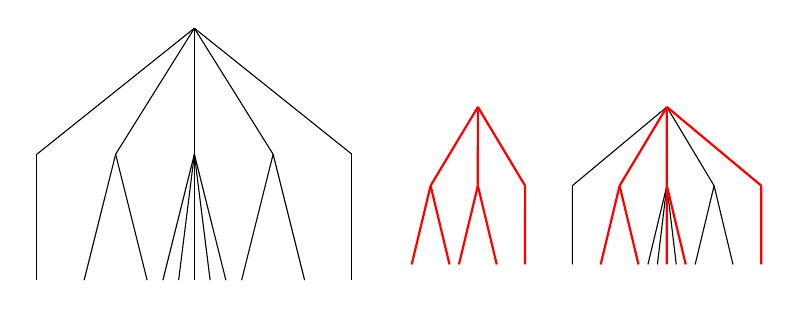
\begin{tikzpicture}
  \begin{scope}[xscale=1,yscale=1.6]
  \path (0,0) node[coordinate] (root) {};
  \foreach \x in {-2,...,2}
    {\draw (root) -- (\x,-1) node[coordinate] (n\x) {};}
  \foreach \s/\x/\n in {-2/-2/,
    -1/-1.4/,-1/-.6/,
    0/-.4/,0/-.2/,0/0/,0/.2/,0/.4/,
    1/.6/,1/1.4/,
    2/2/}
    {\draw (n\s) -- (\x,-2) node[below] {$\n$};}
  \end{scope}

  \begin{scope}[xscale=.6,yscale=1]
  \path (6,-1) node[coordinate] (root) {};
  \foreach \x in {-1,0,1}
    {\draw[red, thick] (root) -- (6+\x,-2) node[coordinate] (m\x) {};}
  \foreach \s/\x in {-1/-1.4,
				    -1/-.6,
				    0/-.4,
				    0/.4,
				    1/1}
    {\draw[red, thick] (m\s) -- (6+\x,-3);}

  \path (10,-1) node[coordinate] (root) {};
  \foreach \x in {-2,1}
    {\draw (root) -- (10+\x,-2) node[coordinate] (o\x) {};}
  \foreach \x in {-1,0,2}
    {\draw[red, thick] (root) -- (10+\x,-2) node[coordinate] (o\x) {};}
  \foreach \s/\x in {-2/-2,
			    0/-.4,
			    0/-.2,
			    0/.2,
			    1/.6,
			    1/1.4}
    {\draw (o\s) -- (10+\x,-3);}
  \foreach \s/\x in {-1/-1.4,
    			-1/-.6,
			    0/0,
			    0/.4,
			    2/2}
    {\draw[red, thick] (o\s) -- (10+\x,-3);}
  \end{scope}
\end{tikzpicture}
\caption{On the left, a tree for $d = 4$, which is the smallest $(5,2)$-universal tree:
it has size $11$ (meaning it has $11$ branches).
On the right, a tree of size $5$ and one possible embedding into the universal tree.}
\label{3-fig:example_universal}
\end{figure*}

We say that a tree $t$ embeds into another tree $T$ if:
\begin{itemize}
	\item either both are leaves,
	\item or let $t = [t_1,\dots,t_k]$ and $T = [T_1,\dots,T_{k'}]$, 
	there exist $i_1 < \dots < i_k$ such that for all $j \in [1,k]$ we have that $t_j$ embeds into $T_{i_j}$.
\end{itemize}

\begin{definition}
A tree is $(n,h)$-\textit{universal} if it embeds all trees of size $n$ and height $h$.
\end{definition}

We refer to \cref{3-fig:example_universal} for an example of a $(5,2)$-universal tree.
A first example of an $(n,h)$-universal tree is the tree where each node has degree $n$:
formally we define it recursively by $T_{n,0}$ is a leaf, and $T_{n,h+1} = [\underbrace{T_{n,h},\dots,T_{n,h}}_{n \text{ copies}}]$.
It has size $n^h$.

\subsubsection*{A quasipolynomial universal tree}
We present an inductive construction of a quasipolynomial universal tree.

\begin{theorem}
\label{3-thm:universal_tree}
There exists an $(n,h)$-universal tree with size $f(n,h)$, where $\mu$ satisfies the following:
$$\begin{array}{lll}
f(n,h) & = & f(n,h-1) + f(\lfloor n/2 \rfloor,h) + f(\lceil n/2 \rceil - 1,h), \\
f(n,1) & = & n, \\
f(1,h) & = & 1.
\end{array}$$
%Furthermore, all $(n,h)$-universal trees have size at least $g(n,h)$,
%where $\frac{f(n,h)}{g(n,h)} = O(nh)$.
\end{theorem}
An upper bound is given by
\[
f(n,h) \le 2n \binom{\lceil \log(n) \rceil + h - 1}{\lceil \log(n) \rceil}.
\]
A generous upper bound on the expression above is $n^{O(\log(h))}$.
A refined analysis reveals that the expression is polynomial in $n$ and $h$ if $h = O(\log(n))$.

%We do not prove the lower bound in this chapter.

\begin{proof}
To construct the $(n,h)$-universal tree $T$, let:
\begin{itemize}
	\item $T_\text{left}$ be a $(\lfloor n/2 \rfloor,h)$-universal tree,
	\item $T_\text{middle}$ be a $(n,h-1)$-universal tree,
	\item $T_\text{right}$ be a $(\lceil n/2 \rceil - 1,h)$-universal tree.
\end{itemize}
The intuitive construction of $T$ is as follows: 
we merge the roots of $T_\text{left}$ and $T_\text{right}$ and insert inbetween them
a child of the root to which is attached $T_\text{middle}$.
Formally, let $T_\text{left} = [T^1_{\text{left}},\dots,T^k_{\text{left}}]$ and 
$T_\text{right} = [T^1_{\text{right}},\dots,T^{k'}_{\text{right}}]$,
we define $T$ as
\[
[T^1_{\text{left}},\dots,T^k_{\text{left}},\ T_\text{middle},\ T^1_{\text{right}},\dots,T^{k'}_{\text{right}}].
\]
The construction is illustrated in \cref{3-fig:smallest_tree_construction}.

\begin{figure}[!ht]
\centering
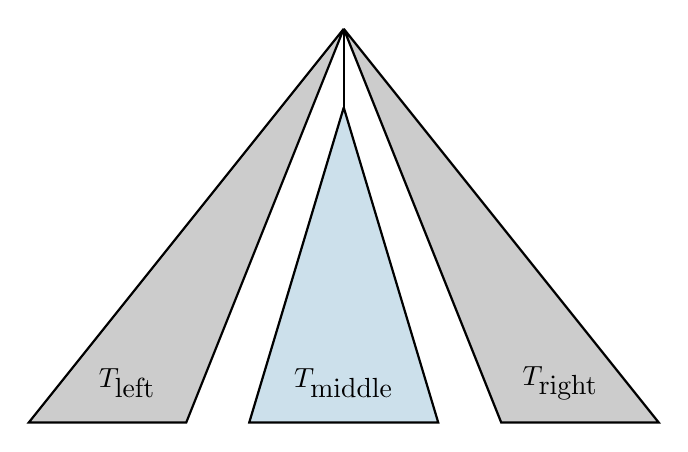
\begin{tikzpicture}
  \begin{scope}[line width=.8pt]
  \foreach \sign/\dir in {-/left,/right}
    {\draw[fill=black!20!white] (0,0) -- (\sign 4,-5) -- (\sign 2,-5) -- (0,0);
     \path (\sign 2.75,-4.5) node {$T_{\textup{\dir}}$};}
  \draw[fill=blue!60!green!20!white] (0,-1) -- (-1.2,-5) -- (1.2,-5) -- (0,-1);
  \path (0,-4.5) node {$T_{\textup{middle}}$};
  \draw (0,0) -- (0,-1);
  \end{scope}
\end{tikzpicture}
\caption{The inductive construction.}
\label{3-fig:smallest_tree_construction}
\end{figure}

\vskip1em
We argue that $T$ is $(n,h)$-universal.
Consider a tree $t = [t_1,\dots,t_k]$ with $n$ branches.
The question is where to cut, \textit{i.e.} which subtree of $t$ gets mapped to $T_\text{middle}$.
Let $n(t_i)$ be the number of branches in $t_i$. 
Since $t$ has $n$ branches, we have $n(t_1) + \cdots + n(t_k) = n$.
There exists a unique $p \in [1,k]$ such that 
$n(t_1) + \cdots + n(t_{p-1}) \le \lfloor n/2 \rfloor
\text{ and } 
n(t_1) + \cdots + n(t_p) > \lfloor n/2 \rfloor$.
The choice of $p$ implies that $n(t_{p+1}) + \cdots + n(t_k) \le \lceil n/2 \rceil - 1$.
To embed $t$ into $T$, we proceed as follows:
\begin{itemize}
	\item the tree $[t_1,\dots,t_{p-1}]$ has at most $\lfloor n/2 \rfloor$ branches,
	so it embeds into $T_\text{left}$ by induction hypothesis;
	\item the tree $t_p$ has height $h-1$ and at most $n$ branches, so in embeds into $T_\text{middle}$ by induction hypothesis;
	\item the tree $[t_{p+1},\dots,t_k]$ has at most $\lceil n/2 \rceil - 1$ branches,
	so it embeds into $T_\text{right}$ by induction hypothesis.
\end{itemize}
\end{proof}
\noindent The construction given in the proof yields the smallest $(5,2)$-universal tree illustrated in \Cref{3-fig:example_universal}.

\subsubsection*{Ordering the branches}
Let us consider a tree $t$.
A branch is given by a list of directions that we define now.
For technical convenience that will manifest itself later, the list of directions is indexed by odd numbers $p \in [1,d]$ downwards:
for example for $d = 10$ a branch is $(D_9,D_7,D_5,D_3,D_1)$.
We often naturally identify a leaf, its branch, and the list of directions that represents it.

We write $B_t$ for the set of branches of $t$ and $\le$ for the lexicographic order on $B_t$.
Note that its interpretation on the tree is: for two branches $b,b'$, we have $b \le b'$ if and only if $b$ is to the left of $b'$.
The strict version of $\le$ is $<$.

We introduce a set of relations $\vartriangleleft_p$ over $B_t$ for each $p \in [1,d]$.
For a branch $b = (D_{d-1},\dots,D_3,D_1)$ we write $b_{\ge p}$ for the tuple $(D_{d-1},\dots,D_{p+2},D_p)$,
which we call the $p$-truncated branch of $b$.
\begin{itemize}
	\item For $p$ odd, we say that $b \vartriangleleft_p b'$ 
	if $b_{\ge p}\ <\ b'_{\ge p}$.
	\item For $p$ even, we say that $b \vartriangleleft_p b'$ 
	if $b_{\ge p}\ \le\ b'_{\ge p}$.
\end{itemize}

To interpret $\vartriangleleft_p$ on the tree, we label the levels by priorities from bottom to top as in \Cref{3-fig:example_universal}.
Then $b \vartriangleleft_p b'$ if and only if the $p$-truncated branch of $b$ is to the left of the $p$-truncated branch of $b'$,
strictly if $p$ is odd, and non-strictly if $p$ is even.

\begin{figure*}[!ht]
\centering
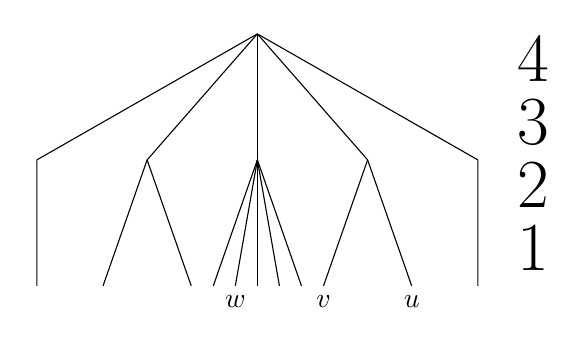
\begin{tikzpicture}
  \begin{scope}[xscale=1.4,yscale=1.6]
  \path (0,0) node[coordinate] (root) {};
  \foreach \x in {-2,...,2}
    {\draw (root) -- (\x,-1) node[coordinate] (n\x) {};}
  \foreach \s/\x/\n in {-2/-2/,
    -1/-1.4/,-1/-.6/,
    0/-.4/,0/-.2/w,0/0/,0/.2/,0/.4/,
    1/.6/v,1/1.4/u,
    2/2/}
    {\draw (n\s) -- (\x,-2) node[below] {$\n$};}
  \foreach \y/\l in {0.2/4,.7/3,1.2/2,1.7/1}
    {\draw (2.5,-\y) node {\begin{Huge}\l\end{Huge}};}
  \end{scope}
\end{tikzpicture}
\caption{Illustration of the relations $\vartriangleleft_p$.}
\label{3-fig:example_relations}
\end{figure*}

We refer to \cref{3-fig:example_relations} for some examples:
\[
v \vartriangleleft_1 u \quad ; \quad  
v \vartriangleleft_2 u \quad ; \quad 
u \vartriangleleft_2 v \quad ; \quad 
w \vartriangleleft_3 u \quad ; \quad 
w \vartriangleleft_2 v.
\]

\begin{lemma}
\label{3-lem:properties_tree}
The relations $\vartriangleleft_p$ for $p \in [1,d]$ induced by a tree $t$ satisfy the following properties:
\begin{itemize}
	\item $\vartriangleleft_d$ is the full relation: for all $b,b'$ we have $b \vartriangleleft_d b'$;
	\item if $b \vartriangleleft_p b'$ and $b' \vartriangleleft_q b''$ then $b \vartriangleleft_{\max(p,q)} b''$;
	\item the relation $\vartriangleleft_p$ is non-reflexive if $p$ is odd;
	\item the relation $\vartriangleleft_1$ is total;
	\item for $p < d$ even we have $b \vartriangleleft_p b'$ if and only if $\neg (b' \vartriangleleft_{p+1} b)$.
\end{itemize}
%Conversely, for any set of relations $\vartriangleleft_p$ for $p \in [1,d]$ over some set $V$ of size $n$ satisfying the properties above,
%there exists a tree $t$ using $V$ as set of leaves inducing these relations.
\end{lemma}
%\begin{proof}
%It is clear that the relations $\vartriangleleft_p$ induced by a tree satisfy the properties.
%
%Conversely, we give an inductive construction.
%Let us assume that the relations $\vartriangleleft_p$ are over the set $V$ of size $n$.
%At any given point we are considering a subset $S$ of $V$ and an odd priority $p$, 
%initially the whole set $V$ and the priority $d-1$.
%Given $S$ and $p$, we partition $S$ as follows:
%$S_1$ is the set of minimal elements from $S$ with respect to $\vartriangleleft_p$, 
%then $S_2$ the set of minimal elements from $S \setminus S_1$ with respect to $\vartriangleleft_p$,
%and so on: $S_k$ is the set of minimal elements from $S \setminus \bigcup_{j < k} S_j$ with respect to $\vartriangleleft_p$.
%We inductively construct the trees associated to each $S_i$ and $p-2$, yielding the tree for $S$ and $p$.
%The fact that the relation $\vartriangleleft_1$ is total implies that the leaves of the tree we construct correspond to singletons of $V$,
%hence can be identified with $V$.
%\end{proof}

The following observation rephrases the notion of embeddings between trees using the ordering on branches.

\begin{fact}
\label{3-fact:embedding}
Let $t,T$ be two trees.
Then $t$ embeds into $T$ if and only if there exists a function $\mu : B_t \to B_T$
such that for all branches $b,b'$:
\[
b \vartriangleleft_p^t b' \implies \mu(b) \vartriangleleft_p^T \mu(b').
\]
\end{fact}

\subsubsection*{Progress measures}
We explain how a tree $t$ induces both a lattice $(Y_t,\le)$ and a monotonic function $\delta_t : Y_t \times [1,d] \to Y_t$.
The set $Y_t$ is the set of branches of $t$ augmented with a new element $\bot$, 
and $\le$ is the lexicographic order on branches with $\bot$ as least element.
For each $p \in [1,d]$ and $b \in Y_t$ we extend $\vartriangleleft_p$ with $\bot \vartriangleleft_p b$.
We then define $\delta : Y_t \times [1,d] \to Y_t$ by
\[
\delta(b,p) = \max \set{b' : b' \vartriangleleft_p b}.
\]
This in turn induces a monotonic operator $\Op_t : F_V \to F_V$ defined by:
\[
\Op(\mu)(v) = 
\begin{cases}
\max \set{\delta( \mu(v'), \col(v)) : (v,v') \in E} & \text{ if } v \in \VE, \\
\min \set{\delta( \mu(v'), \col(v)) : (v,v') \in E} & \text{ if } v \in \VA.
\end{cases}
\]

Let $\Game$ be a parity game, a progress measure is a function $\mu : V \to Y_t$ which is a post-fixed point: $\mu \le \Op_t(\mu)$. 
Expanding the definitions, this means that for all vertices $v$, we have
\[
\begin{array}{llll}
\exists (v,v') \in E,\ & \mu(v) \le \delta_t( \mu(v'), \col(v)) & \text{ if } v \in \VE, \\
\forall (v,v') \in E,\ & \mu(v) \le \delta_t( \mu(v'), \col(v)) & \text{ if } v \in \VA.
\end{array}
\]
The definition of $\delta_t$ further simplifies it to: for all vertices $v$, we have
\[
\begin{array}{llll}
\exists (v,v') \in E,\ & \mu(v) \vartriangleleft_{\col(v)} \mu(v') & \text{ if } v \in \VE, \\
\forall (v,v') \in E,\ & \mu(v) \vartriangleleft_{\col(v)} \mu(v') & \text{ if } v \in \VA.
\end{array}
\]

The following theorem is our first and main step towards proving the characterisation principle.

\begin{theorem}
\label{3-thm:progress_measure}
Let $\Game$ be a parity game and $v$ a vertex.
Then Eve wins from $v$ if and only if there exists a tree $t$ and a progress measure $\mu : V \to Y_t$ such that $\mu(v) \neq \bot$.
\end{theorem}

In order to prove \cref{3-thm:progress_measure}, we first consider the case of parity graphs.
A progress measure in a parity graph is a function $\mu : V \to Y_t$ such that 
for all edges $(v,v') \in E$ we have $\mu(v) \vartriangleleft_{\col(v)} \mu(v')$.

Recall that a graph satisfies parity from $v$ if all infinite paths from $v$ satisfy parity.
This is equivalent to asking whether all cycles reachable from $v$ are even, meaning the maximal priority appearing in the cycle is even.

\begin{lemma}
\label{3-lem:progress_measure}
Let $G$ be a parity graph and $v$ a vertex.
Then $G$ satisfies parity from $v$ if and only if 
there exists a tree $t$ and a progress measure $\mu : V \to Y_t$ such that $\mu(v) \neq \bot$.
\end{lemma}

\begin{proof}
Let us assume that there exists a tree $t$ and a progress measure $\mu : V \to Y_t$ such that $\mu(v) \neq \bot$
and for all edges $(v,v') \in E$ we have $\mu(v) \vartriangleleft_{\col(v)} \mu(v')$.
To show that $G$ satisfies parity from $v$ we show that any cycle reachable from $v$ is even.
Let us consider such a cycle:
\[
(v_1,v_2) (v_2,v_3) \cdots (v_k,v_1).
\]
Since the cycle is reachable from $v$ and $\mu(v) \neq \bot$, this implies that $\mu(v_i) \neq \bot$ for $i \in [1,k]$.
Let us assume towards contradiction that its maximal priority is odd, and without loss of generality it is $\col(v_1)$.
Applying our hypothesis to each edge of the cycle we have
\[
\mu(v_1) \vartriangleleft_{\col(v_1)} \mu(v_2) \vartriangleleft_{\col(v_2)} \cdots 
\vartriangleleft_{\col(v_{k-1})} \mu(v_k) \vartriangleleft_{\col(v_k)} \mu(v_1).
\]
The second item of \cref{3-lem:properties_tree} implies that $\mu(v_1) \vartriangleleft_{\col(v_1)} \mu(v_1)$, 
which contradicts the third item since $\vartriangleleft_{\col(v_1)}$ is non-reflexive given that $\col(v_1)$ is odd.

\vskip1em
Let us now prove the converse implication.
We prove the following property by induction on the number of vertices:
for all graphs satisfying parity (without the usual assumption that every vertex has an outgoing edge),
there exists a tree $t$ and a progress measure $\mu : V \to Y_t$ such that $\mu(v) \neq \bot$
for all vertices~$v \in V$.

There are two cases: either the largest priority $d$ in the graph is even or it is odd.
We write $V_d$ for the set of vertices of priority $d$. 

\vskip1em
\textit{Case $d$ even.}
Let us consider the graph induced by the set of vertices $V \setminus V_d$.
It satisfies parity, so by induction hypothesis there exists a tree $t$ and a progress measure $\mu_d : V \setminus V_d \to Y_t$ 
such that $\mu_d(v) \neq \bot$ for all vertices $v \in V \setminus V_d$.
We extend $\mu_d$ to $\mu : V \to Y_t$: for $v \in V_d$ we let $\mu(v) = \ell_{\max}$ where $\ell_{\max}$ is the maximal element in $Y_t$.
Then $\mu$ is a progress measure such that $\mu_d(v) \neq \bot$ for all vertices $v \in V$.
Indeed the additional edges are of the form $(v,v')$ for either $v \in V_d$ or $v' \in V_d$:
in the first case $\mu(v) \vartriangleleft_{\col(v)} \mu(v')$ holds because $\vartriangleleft_d$ is the full relation,
and in the second case because $\mu(v') = \ell_{\max}$.

\vskip1em
\textit{Case $d$ odd.}
We claim that there exists a non-trivial partition $V = W_1 \uplus W_2$ such that there is no edge from $W_1$ to $W_2$.
Let $u \in V_d$, define $U$ the set of vertices reachable from $u$ by a non-trivial path.
If $U$ is empty, then $V = \set{u} \uplus (V \setminus \set{u})$ is a non-trivial partition as desired.
Otherwise $U$ is non empty, then $V = U \uplus (V \setminus U)$ is a non-trivial partition as desired:
to see that $V \setminus U$ is non empty we note that $u \in V \setminus U$, otherwise there would be an odd cycle 
(containing the maximal and odd priority $d$).

We consider the graphs induced by $W_1$ and $W_2$.
They both satisfy parity, so by induction hypothesis for $i \in \set{1,2}$ 
there exists a tree $t_i$ and a progress measure $\mu_i : W_i \to Y_{t_i}$ 
such that $\mu_i(v) \neq \bot$ for all vertices $v \in W_i$.
We let $t$ denote the tree obtained by putting the two trees $t_1$ and $t_2$ side by side with $t_2$ on the left of $t_1$.
Formally, $t_1 = [t^1_1,\dots,t^k_1]$ and $t_2 = [t^1_2,\dots,t^{k'}_2]$, let 
$t = [t^1_2,\dots,t^{k'}_2,\ t^1_1,\dots,t^k_1]$.
We define $\mu : V \to Y_t$ by $\mu(v) = \mu_i(v)$ if $v \in W_i$.
Then $\mu$ is a progress measure: for edges in the graphs induced by $W_1$ and $W_2$ this is because $\mu_1$ and $\mu_2$ are,
and the additional edges are from $v \in W_2$ to $v' \in W_1$, so indeed $\mu(v) \vartriangleleft_{\col(v)} \mu(v')$ holds.
This finishes the inductive proof of the property.

\vskip1em
We show that the property extends to graphs not satisfying parity.
Let $G$ a parity graph and $W$ the set of vertices $v$ such that $G$ satisfies parity from $v$.
Let $G'$ the graph induced by $W$, it satisfies parity so 
by the property above there exists a tree $t$ and a progress measure $\mu_W : W \to Y_t$ such that
$\mu_W(v) \neq \bot$ for all vertices $v \in W$.
We extend $\mu_W$ to $\mu : V \to Y_t$: for $v \notin W$ we let $\mu(v) = \bot$.
To see that $\mu$ is a progress measure we make two remarks.
First, if $v \in W$ then all successors of $v$ are also in $W$ (by prefix independence of parity),
so the edges in $G$ are either in $G'$ or from $v \in V \setminus W$ to $v' \in W$.
In the first case $\mu(v) \vartriangleleft_{\col(v)} \mu(v')$ holds because $\mu_W$ is a progress measure,
and in the second case because $\mu(v) = \bot$.
\end{proof}

We can now prove \cref{3-thm:progress_measure}.

\begin{proof}
Assume that Eve wins from $v$ and let $\sigma$ be a positional strategy.
The parity graph $\Game[\sigma]$ satisfies parity from $v$, so thanks to \cref{3-lem:progress_measure}
there exists a tree $t$ and a function $\mu : V \to Y_t$ such that $\mu(v) \neq \bot$
and for all edges $(v,v') \in E$ we have $\mu(v) \vartriangleleft_{\col(v)} \mu(v')$.
We remark that $\mu : V \to Y_t$ is actually a progress measure: the condition for $v \in \VE$ is ensured by the edge $\sigma(v)$,
and the condition for $v \in \VA$ by assumption on $\mu$.

\vskip1em
Conversely, assume that there exists a tree $t$ and a progress measure $\mu : V \to Y_t$.
It induces a positional strategy defined by $\sigma(v) = (v,v')$ such that $\mu(v) \vartriangleleft_{\col(v)} \mu(v')$.
We argue that $\sigma$ is a winning strategy from any vertex $v$ such that $\mu(v) \neq \bot$.
This is a consequence of \cref{3-lem:progress_measure} for the parity graph $\Game[\sigma]$.
\end{proof}

\Cref{3-thm:progress_measure} is very close to the characterisation principle we are after,
the only difference being that the lattice $(Y_t,\le)$ depends on an existentially quantified tree $t$.
This is where we use universal trees:

\begin{corollary}
\label{3-cor:progress_measure}
Let $\Game$ be a parity game with $n$ vertices and priorities in $[1,d]$, and $v$ a vertex.
Let $T$ be a $(n,d/2)$-universal tree.
Then Eve wins from $v$ if and only if there exists a progress measure $\mu : V \to Y_T$ such that $\mu(v) \neq \bot$.
\end{corollary}

\begin{proof}
Assume that Eve wins from $v$, thanks to \cref{3-thm:progress_measure} there exists a tree $t$ and a progress measure $\mu : V \to Y_t$ 
such that $\mu(v) \neq \bot$.
Since $T$ is $(n,d/2)$-universal and~$t$ has at most $n$ branches, $t$ embeds into $T$,
which thanks to \cref{3-fact:embedding} implies that there exists $\mu' : B_t \to B_T$ respecting the relations $\vartriangleleft$.
We extend it to $\mu' : Y_t \to Y_T$ by $\mu'(\bot) = \bot$.
Then the composition $\mu' \circ \mu : V \to Y_T$ is a progress measure such that $(\mu' \circ \mu)(v) \neq \bot$. 

The converse implication is a direct consequence of \cref{3-thm:progress_measure}.
\end{proof}

We have proved that the characterisation principle holds for any $(n,d/2)$-universal tree.

\subsection*{The algorithm}
Let us fix $T$ an $(n,d/2)$-universal tree.
It induces both a lattice $(Y_T,\le)$ and a monotonic function $\delta_T : Y_T \times [1,d] \to Y_T$,
which in turn induces a monotonic operator $\Op_T : F_V \to F_V$.
Since $T$ is fixed we do not specify the subscript $T$ for all these objects.

%Thanks to \cref{3-cor:progress_measure} the characterisation principle holds:
%Eve wins from $v$ if and only if there exists a progress measure $\mu : V \to Y$ such that $\mu(v) \neq \bot$.

The last step is to construct an algorithm returning the maximal progress measure relying on Kleene's fixed point theorem (stated as \cref{1-thm:kleene}).
The generic algorithm is explained in \cref{1-sec:value_iteration}, let us instantiate it here.

For the complexity analysis it is useful to decompose $\Op$ into a set of operators:
\[
\Op_v(\mu)(u) = 
\begin{cases}
\mu(v) & \text{ if } u \neq v, \\
\max \set{\delta( \mu(v'), \col(v)) : (v,v') \in E} & \text{ if } u = v \in \VE, \\
\min \set{\delta( \mu(v'), \col(v)) : (v,v') \in E} & \text{ if } u = v \in \VA.
\end{cases}
\]

We introduce some terminology: we say that an edge $e = (v,v')$ is \textit{neglected} if $\neg (\mu(v) \vartriangleleft_{\col(v)} \mu(v'))$,
and a vertex $v$ is \textit{neglected} if $\neg (\mu(v) \le \Op_v(\mu)(v))$.

\begin{figure}[!ht]
\centering
\begin{tikzpicture}
  \node[s-adam] (v) at (0,-2) {$\begin{array}{c} v \\ 3 \end{array}$};
  \node[s-eve] (v') at (2,-1) {$v'$};
  \node[s-eve] (v'') at (2,-3) {$v''$};    

    \path[arrow]
      (v) edge (v')
      (v) edge (v'');

  \begin{scope}[xscale=1.4,yscale=1.6]
  \path (5,0) node[coordinate] (root) {};
  \foreach \x in {-2,...,2}
    {\draw (root) -- (5+\x,-1) node[coordinate] (n\x) {};}
  \foreach \s/\x/\n in {-2/-2/,
    -1/-1.4/,-1/-.6/\Op_v(v),
    0/-.4/,0/-.2/,0/0/,0/.2/v'',0/.4/,
    1/.6/v',1/1.4/,
    2/2/v}
    {\draw (n\s) -- (5+\x,-2) node[below] {$\n$};}

  \node (old) at (5+2,-2.25) {};    
  \node (new) at (5-.6,-2.25) {};    
  \path[arrow]
    (old) edge[bend left, red, thick] (new);

  \foreach \y/\l in {0.2/4,.7/3,1.2/2,1.7/1}
    {\draw (7.5,-\y) node {\begin{Huge}\l\end{Huge}};}
  \end{scope}
\end{tikzpicture}
\caption{The operator $\Op_v$ in action: $\Op_v(\mu)(v)$ is the maximal leaf (meaning the rightmost leaf) 
which satisfies $\Op_v(\mu)(v) \vartriangleleft_3 \mu(v')$ and $\Op_v(\mu)(v) \vartriangleleft_3 \mu(v'')$.}
\label{3-fig:lifting}
\end{figure}

The pseudocode for the algorithm is given in \cref{3-algo:value_iteration}, 
where we let $\ell_{\max}$ denote the maximal leaf in $T$.

\begin{algorithm}[ht]
 \KwData{A parity game with $n$ vertices priorities in $[1,d]$ and a $(n,d/2)$-universal tree $T$.}
 \DontPrintSemicolon

\For{$v \in V$}{
$\mu(v) \leftarrow \ell_{\max}$
}
     
\Repeat{$\forall v \in V,\ \mu \le \Op_v(\mu)$}{
Choose $v \in V$ which is neglected

$\mu \leftarrow \min(\mu, \Op_v(\mu))$}

\Return{$\mu$}
\caption{The value iteration algorithm.}
\label{3-algo:value_iteration}
\end{algorithm}

\begin{theorem}
For all $(n, d/2)$-universal tree $T$, for all parity games $\game$ with $n$ vertices and priorities in $[1,d]$,
the value iteration algorithm over the tree $T$ returns the maximal progress measure $\mu$ for $\game$ over $T$.
\end{theorem}

Thanks to \cref{3-cor:progress_measure}, the maximal progress measure yields a solution for parity games:
Eve wins from $v$ if and only if $\mu(v) \neq \bot$.

\subsection*{Complexity analysis}
The number of times the operator $\Op_v$ is used is bounded by the number of leaves of $T$,
which we write $|T|$, implying that the total number of iterations is bounded by~$n \cdot |T|$.
%This bound cannot be much improved: for instance a vertex of priority $1$ with a self loop is evidently losing but the algorithm
%will use $|T|$ times $\Op_v$ to get this information.
To determine the overall complexity we need to discuss two aspects of the algorithm:
\begin{itemize}
	\item the data structure and in particular the choice of the vertex $v$ in the loop;
	\item the computation of $\Op_v$ and in particular the encoding of branches of $T$.
\end{itemize}

We note that a vertex $v \in \VE$ is neglected if and only if all its outgoing edges are neglected,
and a vertex $v \in \VA$ is neglected if and only if it has a neglected outgoing edge.
Hence checking whether a vertex $v$ is neglected requires considering all of its outgoing edges $(v,v')$
and checking whether $\mu(v) \vartriangleleft_{\col(v)} \mu(v')$.
Let us write $\Delta$ for the complexity of checking whether $\mu(v) \vartriangleleft_{\col(v)} \mu(v')$.
Hence checking whether $v$ is neglected costs 
$O(|\Ing^{-1}(v)| \cdot \Delta)$, where $|\Ing^{-1}(v)|$ is the number of outgoing edges of $v$.

A naive implementation of \cref{3-algo:value_iteration} would in each repeat loop go through every vertex $v$ 
to check whether it is neglected.
This would incur a linear cost: $\sum_{v \in V} O(|\Ing^{-1}(v)| \cdot \Delta) = O(m \cdot \Delta)$.
Thus the overall complexity would be
\[
O((m \cdot \Delta) \cdot (n \cdot |T|)) = O(nm \cdot \Delta \cdot |T|).
\]
Typically $\Delta$ is small (we will see that for a well chosen universal tree $T$ it is polylogarithmic in $n$ and $d$),
and $T$ is the dominating factor (quasipolynomial in $n$ and $d$ thanks to \cref{3-thm:universal_tree}).

We first explain that using a better data structure we can maintain the list of vertices $v$ such that $\neg (\mu \le \Op_v(\mu))$,
saving a linear factor in the complexity.
We then discuss the cost $\Delta$ by choosing an appropriate encoding of the quasipolynomial universal tree constructed in~\cref{3-thm:universal_tree}.

\subsubsection*{Data structure}
We use a data structure similar to the attractor computation presented in \cref{2-sec:attractors}.
The pseudocode is given in \cref{3-algo:value_iteration_data_structure}.
We did not provide the pseudocode for the functions $\texttt{Init}$ and $\texttt{Update}$.

The data structure consists of the following objects:
\begin{itemize}
	\item a leaf of $T$ for each vertex, representing the current function $\mu : V \to Y$;
	\item a set $S$ of vertices (each vertex appears at most once in $S$, the order in which vertices are stored and retrieved from the set does not matter);
	\item for each vertex of Eve a number of edges.
\end{itemize}
For our complexity analysis we use the unit cost RAM model, see \cref{1-sec:computation} for details.
In the case at hand let us choose for the machine word size $w = \log(m) + \log(d)$, 
so that an edge together with its priority can be stored in one machine word.
The space complexity of this data structure depends on the encoding of $T$, which we will discuss later.

The invariant of the algorithm satisfied before each iteration of the repeat loop is the following:
\begin{itemize}
	\item for $v \in \VA$, the value of $\text{number}$-$\text{neglected}$-$\text{edges}(v)$
	is the number of neglected edges of $v$;
	\item $S$ is the set of neglected vertices.
\end{itemize}
The invariant is satisfied initially thanks to the function $\texttt{Init}$.
Let us assume that we choose and remove $v$ from $S$.
Since we modify only $\mu(v)$ the only potentially neglected vertices are in $S$ (minus $v$) and the incoming edges of $v$;
for the latter each of them is checked and added to $S$ when required.
By monotonicity, neglected vertices remain neglected so all vertices in $S$ (minus $v$) are still neglected.
Hence the invariant is satisfied.

The invariant implies that the algorithm indeed implements~\cref{3-algo:value_iteration} hence returns the maximal progress measure, 
but it also has implications on the complexity.
Indeed one iteration of the repeat loop over some vertex $v$ involves 
\[
O\left( (|\Ing^{-1}(v)| + |\Out^{-1}(v)|) \cdot \Delta \right)
\]
operations,
the first term corresponds to updating $\mu(v)$ and $\text{number}$-$\text{neglected}$-$\text{edges}(v)$,
which requires for each outgoing edge of $v$ to compute $\delta$,
and the second term corresponds to considering all incoming edges of $v$ and treating the neglected ones.
Thus the overall complexity is
\[
O\left( 
\sum_{v \in V} (|\Ing^{-1}(v)| + |\Out^{-1}(v)|) \cdot \Delta \cdot |T|
\right) 
= O(m \cdot \Delta \cdot |T|).
\]

\begin{algorithm}
 \KwData{A parity game with $n$ vertices priorities in $[1,d]$ and a $(n,d/2)$-universal tree $T$.}
 \SetKwFunction{FTreat}{Treat}
 \SetKwFunction{FVI}{ValueIteration}
 \SetKwFunction{FInit}{Initialise}
 \SetKwFunction{FUpdate}{Update}
 \SetKwProg{Fn}{Function}{:}{}
 \DontPrintSemicolon
 
\Fn{\FVI{}}{
%	\For{$v \in V$}{
%		$\mu(v) \leftarrow \ell_{\max}$
%	}
	
	\FInit{$\mu$, $\text{number}$-$\text{neglected}$-$\text{edges}$, $S$}

%	\vskip1em
%	\For{$e \in E$}{	
%		\If{$e$ is neglected}{
%			\FTreat($e$)
%		}
%	}

	\vskip1em
	\Repeat{$S$ empty}{
		Choose some $v$ in $S$ and remove it from $S$

		$\mu \leftarrow \min(\mu, \Op_v(\mu))$

		\FUpdate{$\text{number}$-$\text{neglected}$-$\text{edges}(v)$}

		\For{$e \in E$ \text{ such that } $\Out(e) = v$}{
			\If{$e$ is neglected}{
				\FTreat($e$)
			}
		}
	}

	\Return{$\mu$}
}

\vskip1em
\Fn{\FTreat{$e$}}{
	$v \leftarrow \Ing(e)$
	
	\If{$v \in \VA$ and $v \notin S$}{
		Add $v$ to $S$		
	}
	
	\If{$v \in \VE$ and $v \notin S$}{	
		$\text{number}$-$\text{neglected}$-$\text{edges}(v) \leftarrow \text{number}$-$\text{neglected}$-$\text{edges}(v) + 1$

		\If{$\text{number}$-$\text{neglected}$-$\text{edges}(v) = $ number of outgoing edges of $v$}{
			Add $v$ to $S$
		}
	}
}
\caption{The value iteration algorithm with explicit data structure.}
\label{3-algo:value_iteration_data_structure}
\end{algorithm}

\subsubsection*{Encoding branches}
Let us fix $T$ to be the quasipolynomial universal tree constructed in \cref{3-thm:universal_tree}.

In our definition of trees we say that a tree is an ordered list of subtrees $[t_1,\dots,t_k]$,
so we use $[1,k]$ with the natural order for ordering the subtrees.
Any other total order can be used to that effect, and a more appropriate order may lead to smaller encoding.
Indeed, using $[1,k]$ for ordering subtrees, if a tree has height $h$ and $n$ branches then a branch is a sequence of $h$ numbers in $[1,n]$,
so it uses $O(h \log(n))$ bits.

Let us consider an order well suited for encoding $T$.
We use $\set{0,1}^*$ the set of binary words and order them using the following three rules that apply for any $u,v \in \set{0,1}^*$:
\[
0u < \varepsilon < 1u \quad ; \quad (0u < 0v \Longleftrightarrow u < v) \quad ; \quad (1u < 1v \Longleftrightarrow u < v).
\]
For words of length at most $2$ the order is $00 < 0 < 01 < \varepsilon < 10 < 1 < 11$.

\begin{figure}[!ht]
\centering
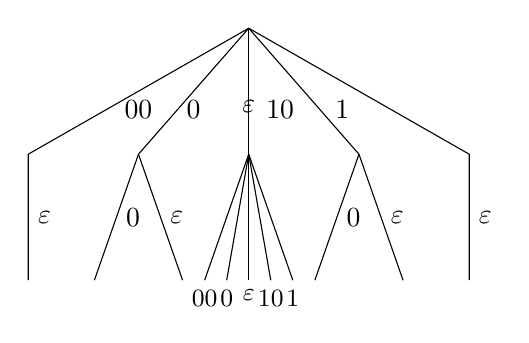
\begin{tikzpicture}
  \begin{scope}[xscale=1.4,yscale=1.6]
  \path (0,0) node[coordinate] (root) {};
  \foreach \x/\n in {-2/00,
  				-1/0,
  				0/\varepsilon}
    {\draw (root) -- node[below] {$\n$} (\x,-1) node[coordinate] (n\x) {};}
  \foreach \x/\n in {1/10,
  				2/1}
    {\draw (root) -- node[below left] {$\n$} (\x,-1) node[coordinate] (n\x) {};}

  \foreach \s/\x/\n in {-2/-2/\varepsilon,
					-1/-1.4/0,
					-1/-.6/\varepsilon,
    				1/.6/0,
    				1/1.4/\varepsilon,
    				2/2/\varepsilon}
    {\draw (n\s) -- node[right] {$\n$} (\x,-2);}
  \foreach \s/\x/\n in {0/-.4/00,
				    0/-.2/0,
				    0/0/\varepsilon,
				    0/.2/10,
				    0/.4/1}
    {\draw (n\s) -- (\x,-2) node[below] {\begin{small}$\n$\end{small}};}
  \end{scope}
\end{tikzpicture}
\caption{The succinct encoding on the $(5,2)$-universal tree.}
\label{3-fig:tree_encoded}
\end{figure}

We can now revisit the construction of the universal tree by defining directly the set of branches.
Recall that $T$ is obtained from $T_\text{left},T_\text{middle}$, and $T_\text{right}$. 
By induction hypothesis branches in $T_\text{left}$ and $T_\text{right}$ are tuples of length $h-1$
and branches in $T_\text{middle}$ tuples of length $h$.
The branches of $T$ are:
\begin{itemize}
	\item branches of $T_\text{left}$ where the first component is prefixed with a $0$;
	\item branches of $T_\text{middle}$ augmented with a new component $\varepsilon$;
	\item branches of $T_\text{right}$ where the first component is prefixed with a $1$.
\end{itemize}
We call this encoding the ""succinct encoding"", it is illustrated in \cref{3-fig:tree_encoded} for the $(5,2)$-universal tree.
The leftmost branch is $(00,\varepsilon)$, and the middle branch $(\varepsilon,\varepsilon)$.
In general, the inductive construction implies that every branch is a tuple $(D_{d-1},\dots,D_1)$ 
such that the sum of the lengths of the directions $D_i$ is at most $\log(n)$.
Thus a branch is encoded using $O(\log(h) \log(n))$ bits: for each of the $\log(n)$ bits we need $\log(h)$ bits to specify its component.

In terms of machine words of size $w = \log(n) + \log(d)$, this means that a branch can be stored using $\log(d)$ machine words.
Hence the data structure uses $O(n \log(d))$ machine words, with together with the input size $O(m)$
means that the space complexity of the algorithm is $O(m + n \log(d))$.

\vskip1em
Using the succinct encoding and a tedious but simple case analysis we can compute $\delta(b,p)$ in time $O(\log(n) \log(d))$.
Putting everything together we obtain the overall complexity 
\[
O\left(nm \log(n) \log(d) \cdot  \binom{\lceil \log(n) \rceil + d/2 - 1}{\lceil \log(n) \rceil} \right),
\]
as stated in \cref{3-thm:value_iteration_quasipoly}.
